\subsubsection{End-to-End Training Time}
\label{sec:e2e-time}

We measure end-to-end training time as the total simulated wall-clock time reported by each experiment, which includes local training, encryption, server-side aggregation, and ciphertext transmission.
This is distinct from the pure serial communication latency (\texttt{TT}) used in Table~\ref{tab:comm-comparison}, which only counts $\sum \max_i t_{\mathrm{up}}^{(i)} + \sum \max_i t_{\mathrm{down}}^{(i)}$.

\textbf{Overall comparison.}
Figure~\ref{fig:e2e-total-time} compares the total training time across the four datasets.
ECPFL-RK on MNIST (130\,s), FMNIST (96\,s) and FedPHE on CIFAR-10 (1221\,s) are the fastest. ECPFL-RK is 1.2$\times$--3.0$\times$ faster than FedAvg+CKKS on these three datasets. On SVHN, ECPFL-RK finishes 2218\,s earlier than FedAvg+CKKS (3.4$\times$ faster). MASER is only 1.1$\times$--1.5$\times$ slower than FedAvg+CKKS (1.3$\times$ on average) in simulated wall-clock time, because the dominant cost of its multi-key CKKS partial-decryption protocol is server-side cryptographic overhead not fully captured by the per-client simulated-time components.

\begin{figure}[t]
\centering
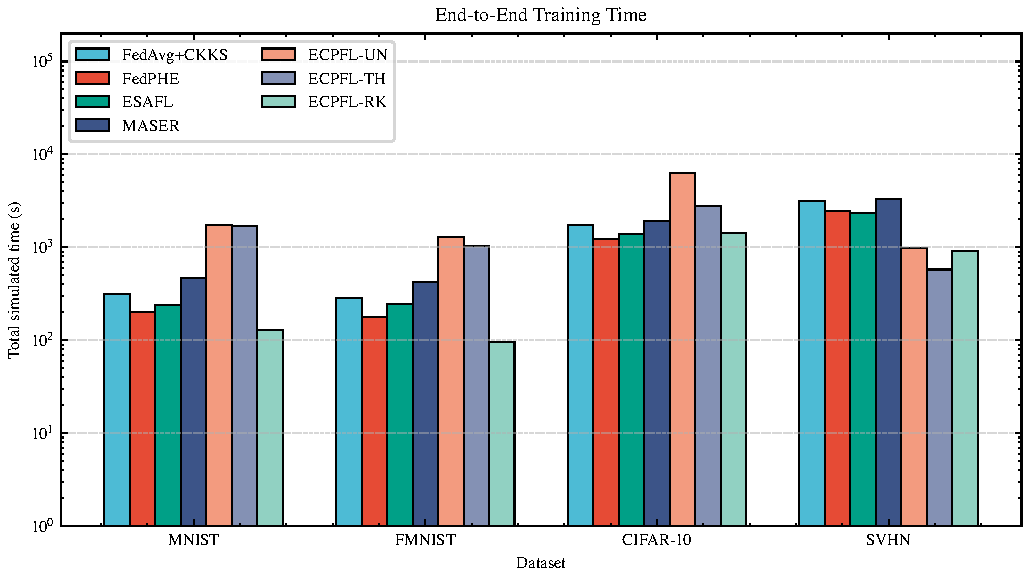
\includegraphics[width=0.95\linewidth]{pic/e2e_total_time.pdf}
\caption{End-to-end training time across datasets and methods. Values are total simulated wall-clock times over 50 rounds.}
\label{fig:e2e-total-time}
\end{figure}

\textbf{Communication bottleneck.}
To understand how much of the wall-clock cost is pure network transfer, Figure~\ref{fig:e2e-comm-time} reports the serial communication time ($\sum \max_i t_{\mathrm{up}}^{(i)} + \sum \max_i t_{\mathrm{down}}^{(i)}$).
ECPFL-RK reduces this metric relative to FedAvg+CKKS by 2.0$\times$--7.7$\times$ (5.0$\times$ on average), cutting MNIST/FMNIST transfers from 452/411\,s to 81/53\,s and the SVHN transfer from 3660\,s to 792\,s. ECPFL-TH obtains comparable or larger reductions on CIFAR-10 and SVHN (4.5$\times$ and 7.5$\times$, respectively), although its more aggressive thresholding is less effective on the smaller datasets. MASER's pure network time is not the dominant factor (463--3956\,s); the gap in Figure~\ref{fig:e2e-total-time} therefore stems from unmeasured server-side multi-key CKKS aggregation and partial-decryption overhead, which we subsume under the residual wall-clock term.

\begin{figure}[t]
\centering
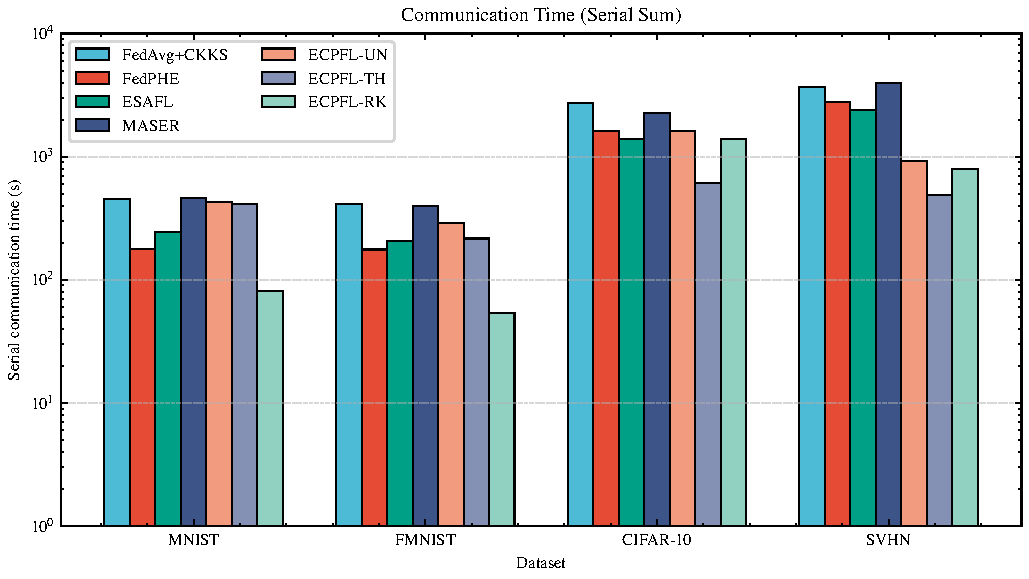
\includegraphics[width=0.95\linewidth]{pic/e2e_comm_time.pdf}
\caption{Serial communication time across datasets and methods.}
\label{fig:e2e-comm-time}
\end{figure}

\textbf{Compute--communication trade-off.}
Figure~\ref{fig:e2e-tradeoff} places every (method, dataset) pair in the compute--communication plane.
The diagonal dashed line marks equal compute and communication time.
FedAvg+CKKS, FedPHE, and ESAFL cluster in the upper-right region, where serial communication exceeds local computation; this confirms that the network is their primary bottleneck. ECPFL variants shift leftward and slightly upward: their serial communication drops sharply, while their compute time increases modestly (average 181\,s for ECPFL-RK versus 165\,s for FedAvg+CKKS) because of additional encryption and prefetch operations. MASER lies off the diagonal in a different way: its measured compute and communication are comparable to the baselines, yet its end-to-end time is larger, again indicating that the dominant cost is server-side cryptographic overhead not captured by the per-client compute components.

\begin{figure}[t]
\centering
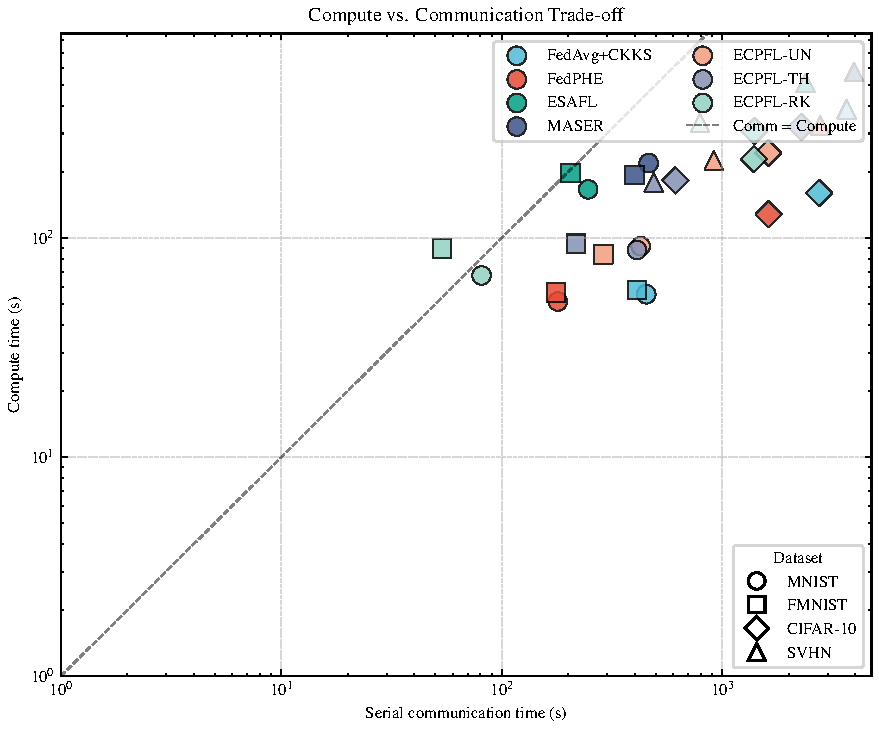
\includegraphics[width=0.8\linewidth]{pic/e2e_tradeoff.pdf}
\caption{Compute versus serial communication time. Each point corresponds to one method--dataset pair. The dashed line represents equal compute and communication time.}
\label{fig:e2e-tradeoff}
\end{figure}
